

\chapter{\Large Cadre général du projet et étude de l'existant}

%Intro\footnotemark\\
%note en bas de page

\textbf{\huge Introduction} \\[0.3cm]



%inclusion d'une mage dans le document
%\begin{figure}[!h]
%\begin{center}
%taille de l'image en largeur
%remplacer "width" par "height" pour régler la hauteur
%\includegraphics[width=15cm]{presentation/schema}
%\end{center}
%légende de l'image
%\caption{Schéma descriptif}
%\end{figure}

%Contenu de la note précédemment marquée avec \footnotemark
%\footnotetext{Note bas de page "intro"}

\scalefont{1.1}  Ce chapitre est consacré à la présentation du cadre général de notre projet. En premier lieu, nous présentons la société d’accueil. Par la suite, nous présentons le cadre du projet qui explique la problématique . Après, on définit par une présentation de la méthodologie que nous allons adopter pour le développement de notre projet. On finit par la présentation des solutions existantes sur le marché avec une étude comparative de ces dernières et présentation de la solution proposée.

%retour à la ligne (alinea)

%saut de paragraphe

%\newpage
%\section{\fontfamily{ptm}\selectfont\Large Cadre général du projet}
\section{\fontfamily{ptm}\selectfont\Large Société d’accueil }
%\textsf{\fontfamily{ptm}\selectfont\scalefont{1.3}Dans ce qui suit,nous présentons la société d'accueil ainsi que son domaine d'activié.}
%\section{\fontfamily{ptm}\selectfont\Large   Identité }
 Mobelite est une agence spécialisée dans le conseil en stratégie mobile, la conception et le développement d’applications mobiles , de sites web et le marketing mobile. Mobelite est forte d’une équipe d’experts dans la réalisation d’applications mobiles sur les platefores les plus répandues et les applications Web. Mobelite dispose d’équipes commerciales et marketing à Paris (France), et d’équipes de développement à Tunis et Monastir (Tunisie).
%\begin{figure}[H]
 %   \begin{center}
    
%    \fbox{
\includegraphics[width=10cm]{presentation/logomob.png}}

 %   \end{center}
    
 %   \caption{Logo de la société mobelite}
%\end{figure}
%\newpage
Ainsi, Mobelite est une société experte dans le création des sites web intuitifs et ergonomiques pour tous les supports soit desktop, tablette ou mobile et avec les plus récentes technologies et Framework de développement comme React JS, Node JS et Angular.Les équipes de mobelite maîtrisent parfaitement la conception et le développement d’applications natives iOS et Android pour tous les différents supports que ce soit smartphone, tablette, Watch et TV. Mobelite excelle dans le conseil de ses clients dans différentes parties de projets comme l'analyse des besoins, UX/UI, la conception, le design,le développement, SEO, DevOps et l'hébergement. Tout ça est réalisé selon la méthodologie Agile, afin de maximiser les possibilités d’itérations sur le concept, et d’introduire plus de flexibilité sur les arbitrages fonctionnels à faire(voir figure 1.2).\\[0.3cm]

\begin{figure}[H]
    \centering
    \fbox{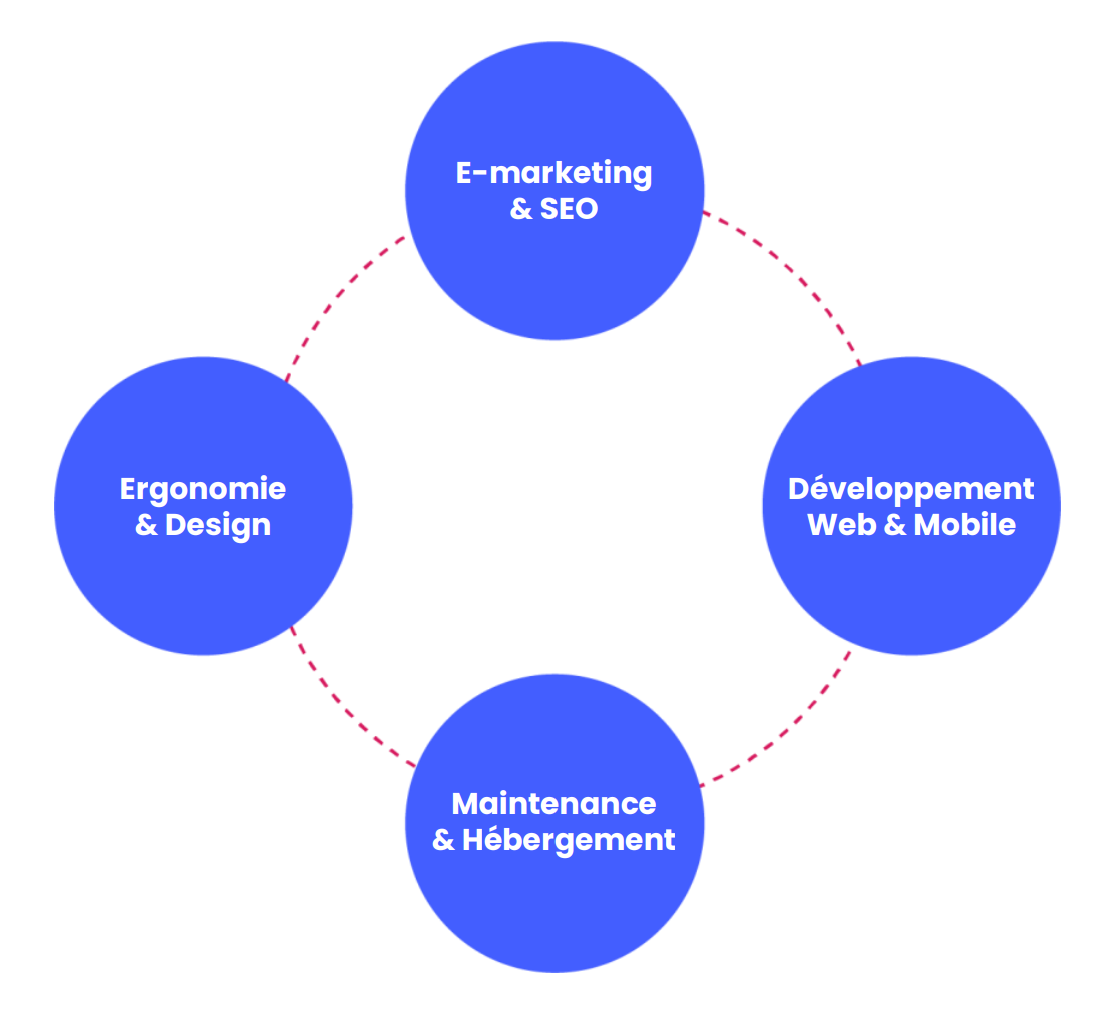
\includegraphics[width=12cm]{presentation/domaine.png}}
    \caption{différents domaines de mobelite}
\end{figure}

\section{\fontfamily{ptm}\selectfont\Large Problématique }
Le déploiement des systèmes de gestion de code source tells que Nexus, SonarQube ou le Monitoring sur un seul serveur local présente plusieurs problèmes qui affectent la performance de serveur et qui rendent l’exécution des diffèrentes applications ou l’ajout des nouvelles fonctionnalités plus difficile . Aussi, la maintenance de plusieurs applications en même temps sera compliquée et nécessite une planification minutieuse pour éviter l’interruption des processus d’autres applications. Les besoins d’entreprise changent au cours des temps et la capacité d'un seul serveur sera insuffisante pour rependre à la charge des données. Les mise à jour des applications peuvent impacter d'autres applications à cause de limites des ressources. En terme de sécurité, une attaque sur le serveur cause une perte des données très grande que sera difficile de récupérer en conséquence de l’utilisation d'un seul serveur.
C'est dans ce cadre que la société souhaite créer son propre solution .
\section{\fontfamily{ptm}\selectfont\Large Notions de base}
 Dans ce qui suit,nous présentons les notions de base que nous utiliserons pour réaliser le projet.
\subsection{\fontfamily{ptm}\selectfont\Large  Microservice}
    Avant l'apparition de l'architecture micro-service, les applications sont construites de manière monolithique, qui est considérée aujourd’hui comme méthode impertinente. L’utilisation de l'architecture monolithique, rend l’application très
    volumineuse avec des difficultés à enrichir les fonctions et le traitement des problèmes.
    Les microservices créent une application unique à partir de plusieurs petits services reliés de manière flexible.
    Ces services ont leur propre logique et leur propre base de données pour un usage spécifique. Chaque service peut être développé, mis à jour, déployé et mis à l’échelle sans affecter les autres services. Les mises à jour logicielles peuvent être plus fréquentes, ce qui améliore la fiabilité, la disponibilité et les performances(Voir figure 1.3). 

\begin{figure}[H]
    \begin{center}
    \fbox{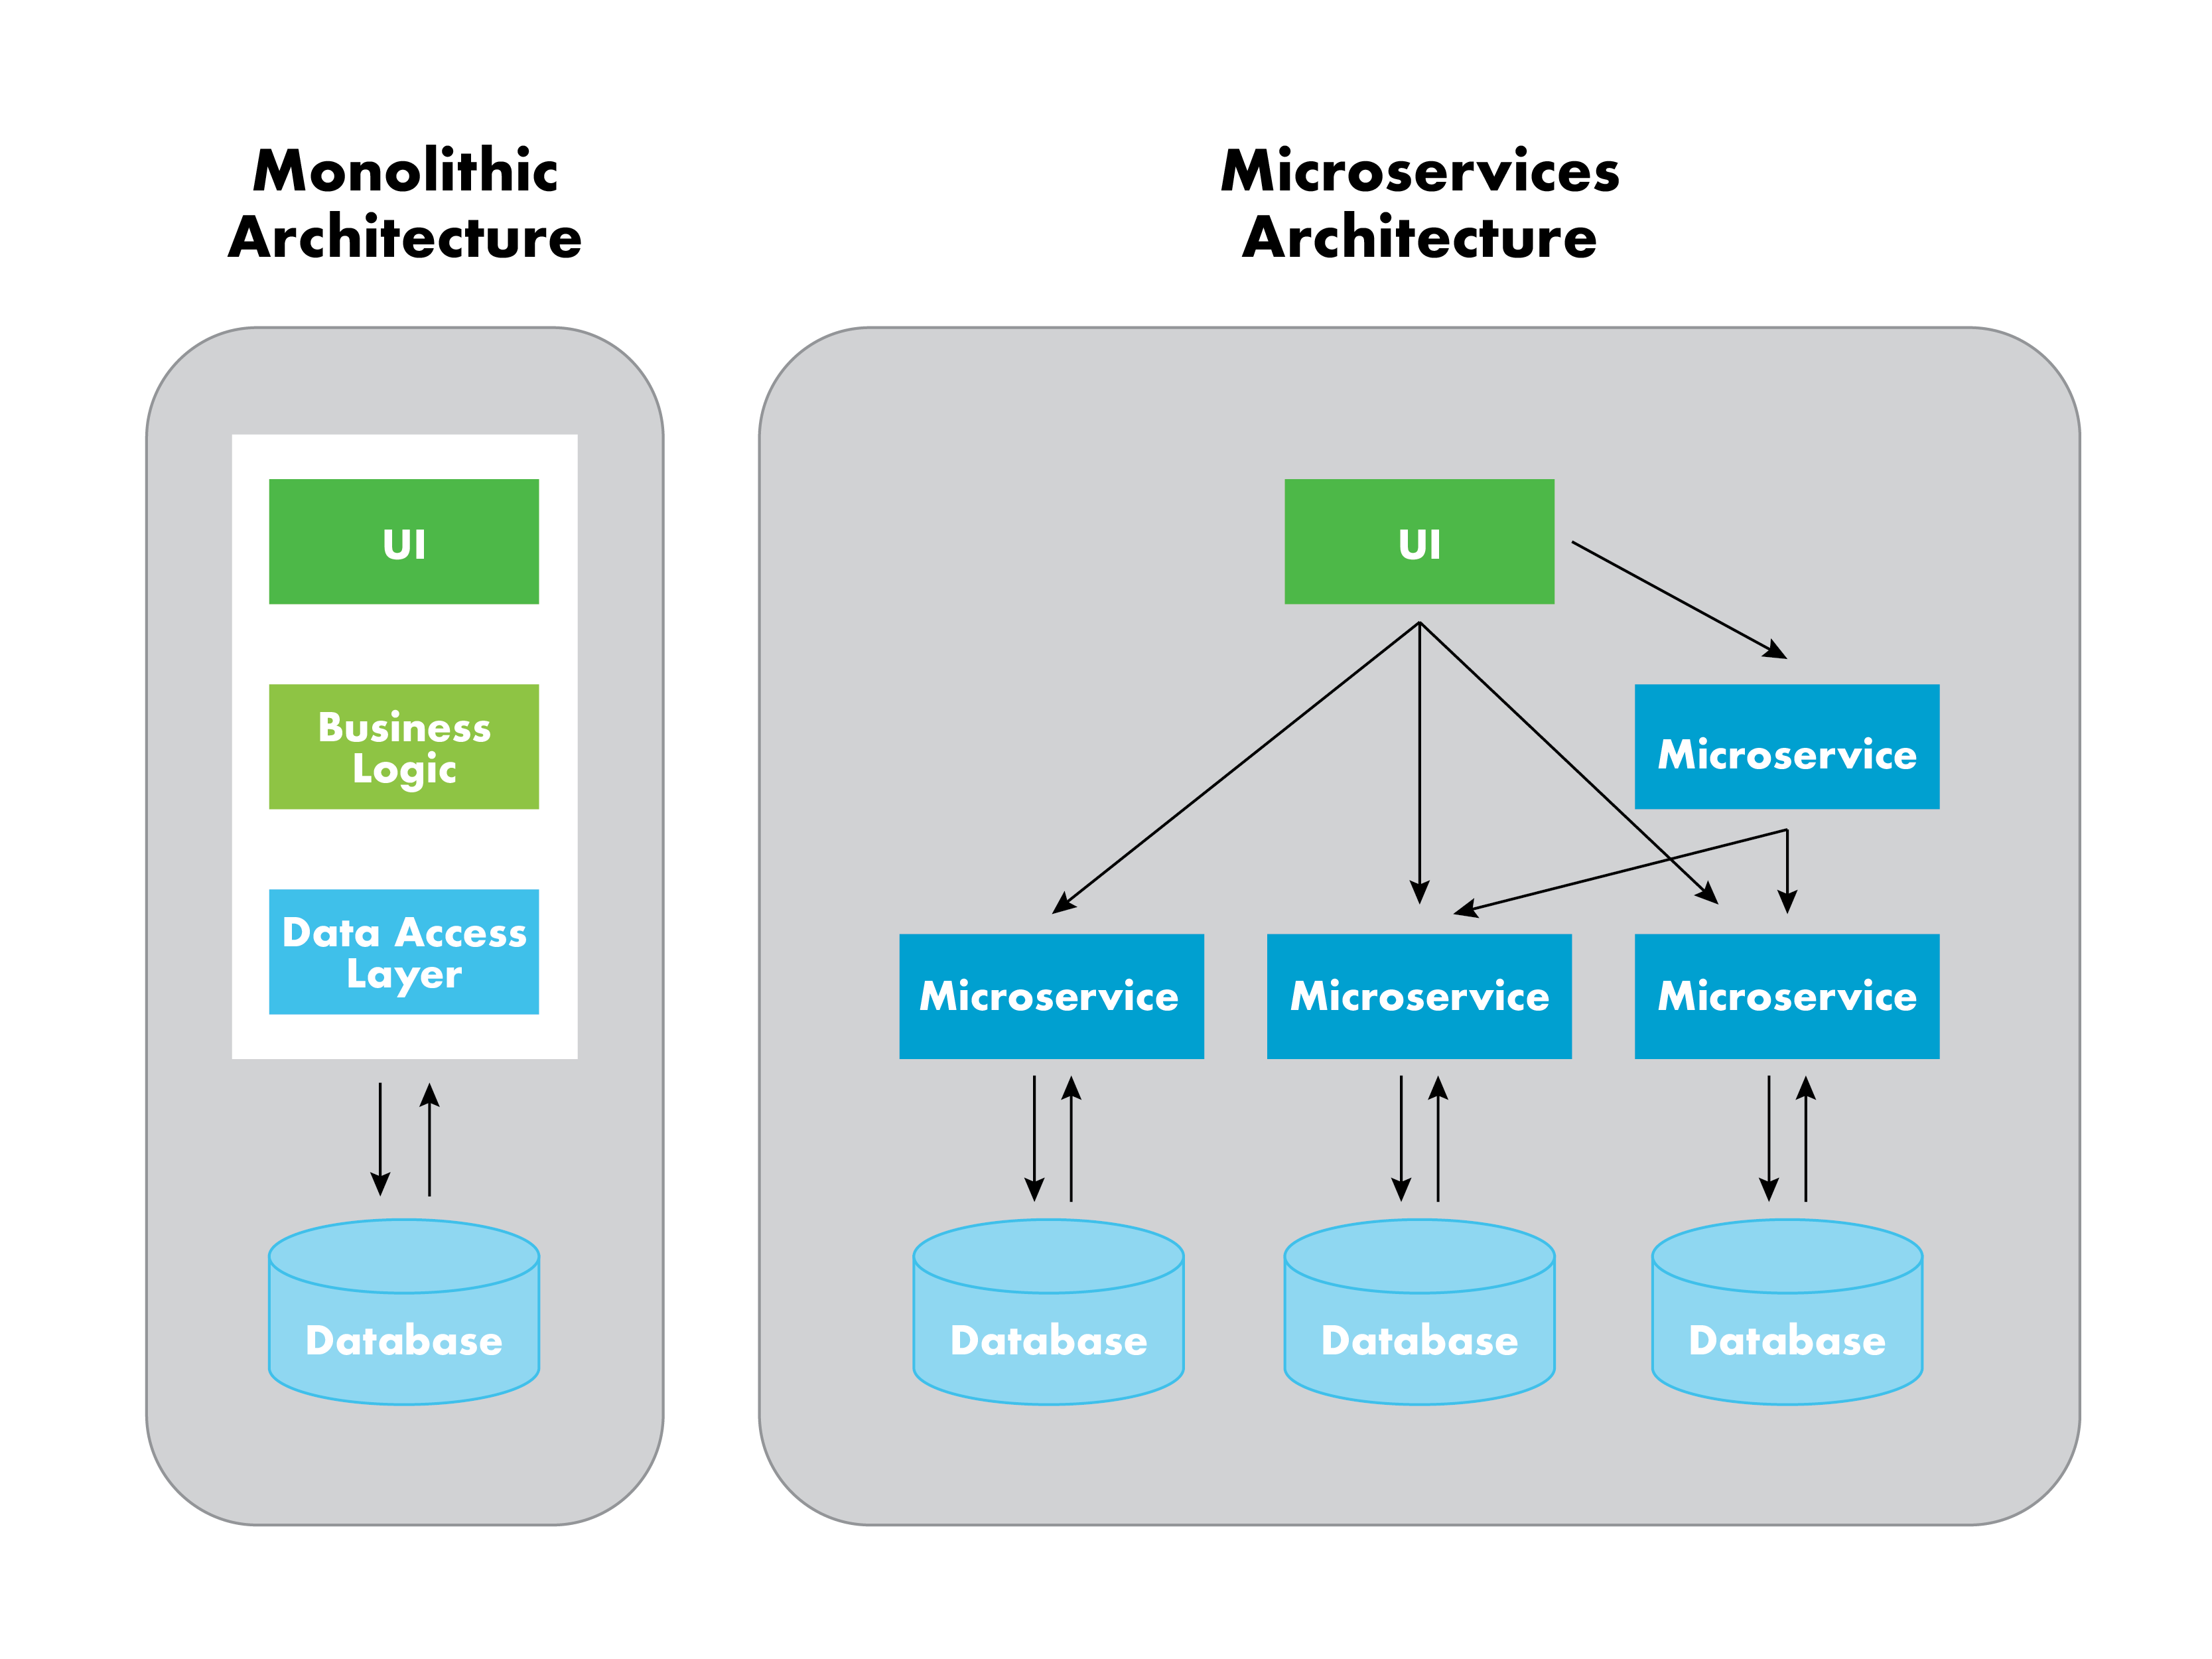
\includegraphics[height=11cm]{presentation/Microservice.png}}
    \end{center}
    \caption{Architecture monolithique vs Micro services}
\end{figure}
\subsection{\fontfamily{ptm}\selectfont\Large  DevOps}

    Combinant développement (Dev) et opérations (Ops), DevOps est l'union des personnes, des processus et des technologies destinés à fournir continuellement de la valeur aux clients.
    DevOps permet la coordination et la collaboration des rôles autrefois cloisonnés (développement, opérations informatiques, ingénierie qualité et sécurité) pour créer des produits plus performantes et plus fiables. En adoptant une culture DevOps ,ainsi que des pratiques et outils DevOps, les équipes peuvent mieux répondre aux besoins des clients, accroître la confiance suscitée par les applications qu'elles développent, et atteindre plus rapidement les objectifs de leur entreprise \cite{1} (voir figure 1.4).
    \begin{figure}[H]
    \begin{center}

    \fbox{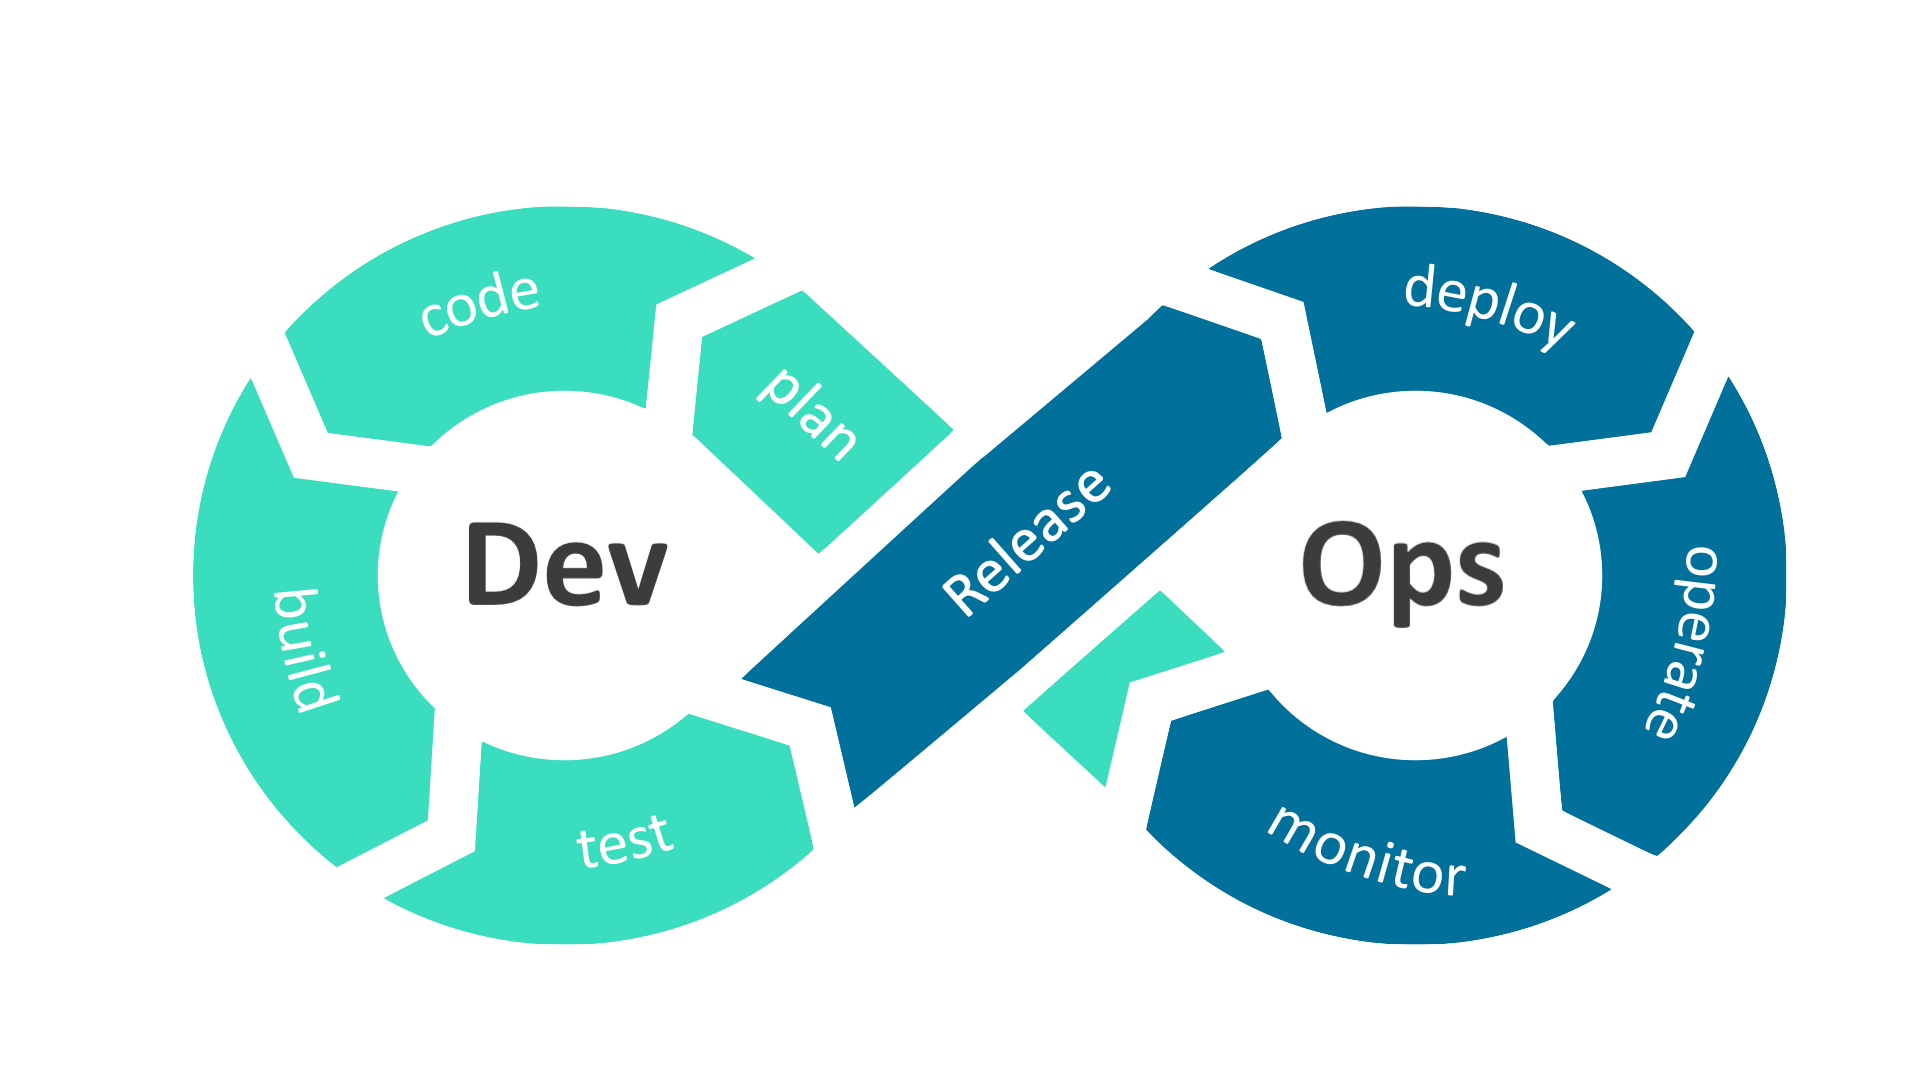
\includegraphics[height=8cm]{presentation/devops.png}}
    \end{center}

    \caption{Cycle de vie DevOps}
\end{figure}
%\textsf{}\\[0.1cm]
\subsection{\fontfamily{ptm}\selectfont\Large  Cloud}

 Le cloud n’est pas une entité physique, mais un vaste réseau de serveurs distants éparpillés tout autour de la planète, reliés entre eux, et destinés à fonctionner comme un écosystème unique. Ces serveurs sont conçus pour stocker et gérer des données, exécuter des applications, ou fournir du contenu ou des services (vidéos diffusées en continu, courrier web, logiciels bureautiques de productivité et autres réseaux sociaux). Au lieu d’accéder à des fichiers et données stockées sur un ordinateur local ou personnel, vous accédez à ces ressources en ligne à partir de n’importe quel appareil compatible avec Internet : les informations sont disponibles en tout lieu et tout le temps.\cite{2} 
\subsubsection{\fontfamily{ptm}\selectfont\Large Modèles de services }

Il existe 3 modèles de services sur le cloud:\\[0.1cm]
\par \noindent \textbf{\Large -Software as a Service (SaaS): }Le Software as a Service, également connu sous le nom de SaaS, est un service basé sur le cloud où, au lieu de télécharger un logiciel que votre PC de bureau ou votre réseau professionnel peut exécuter et mettre à jour, vous accédez à une application via un navigateur internet. L'application logicielle peut être un logiciel de bureautique ou de communication unifiée parmi un large éventail d'autres applications professionnelles disponibles\cite{3} (voir figure 1.4).
%\begin{figure}[H]
%    \begin{center}
%\fbox{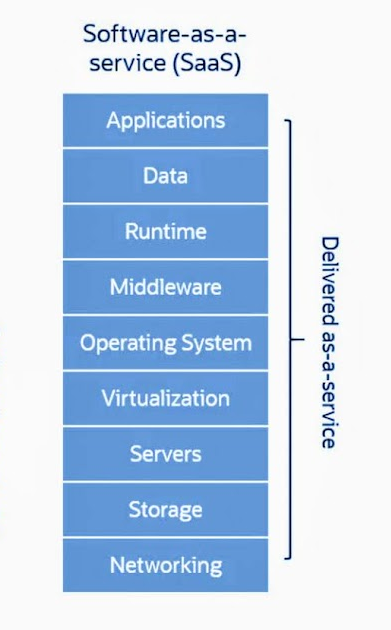
\includegraphics[height=8cm]{presentation/saas.png}}
%    \end{center}

%    \caption{ Architecture SaaS
%    }
%\end{figure}
\noindent \textbf{\Large -Platform as a Service (PaaS): } La Platform-as-a-service (PaaS) est un type d'offre de cloud computing dans lequel un fournisseur de services fournit une plateforme à ses clients, leur permettant de développer, d'exécuter et de gérer des applications commerciales sans avoir à construire et à maintenir l'infrastructure que ces processus de développement de logiciels requièrent généralement(Voir figure 1.4)\cite{4}.\\[0.1cm]
%\begin{figure}[H]
%    \begin{center}
%
%    \fbox{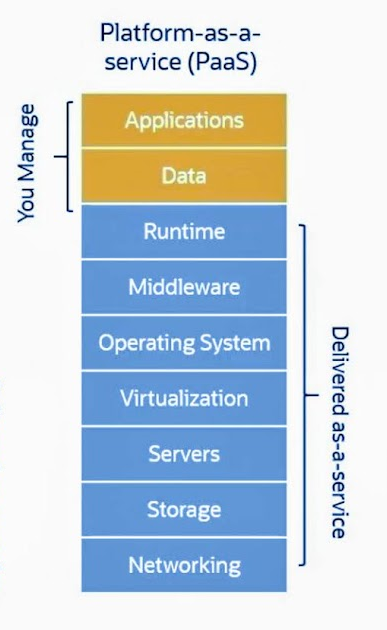
\includegraphics[height=8cm]{presentation/paas.png}}
%    \end{center}
%
%    \caption{ Architecture PaaS}
%\end{figure}
\noindent \textbf{\Large -Infrastructure as a Service (IaaS): }Infrastructure as a service (IaaS) est un type de service de cloud computing qui offre des ressources de calcul, de stockage et de mise en réseau essentielles à la demande, et sur une base de paiement à l’utilisation(Voir figure 1.4)\cite{5}.\\[0.1cm]
\begin{figure}[H]
    \begin{center}

    \fbox{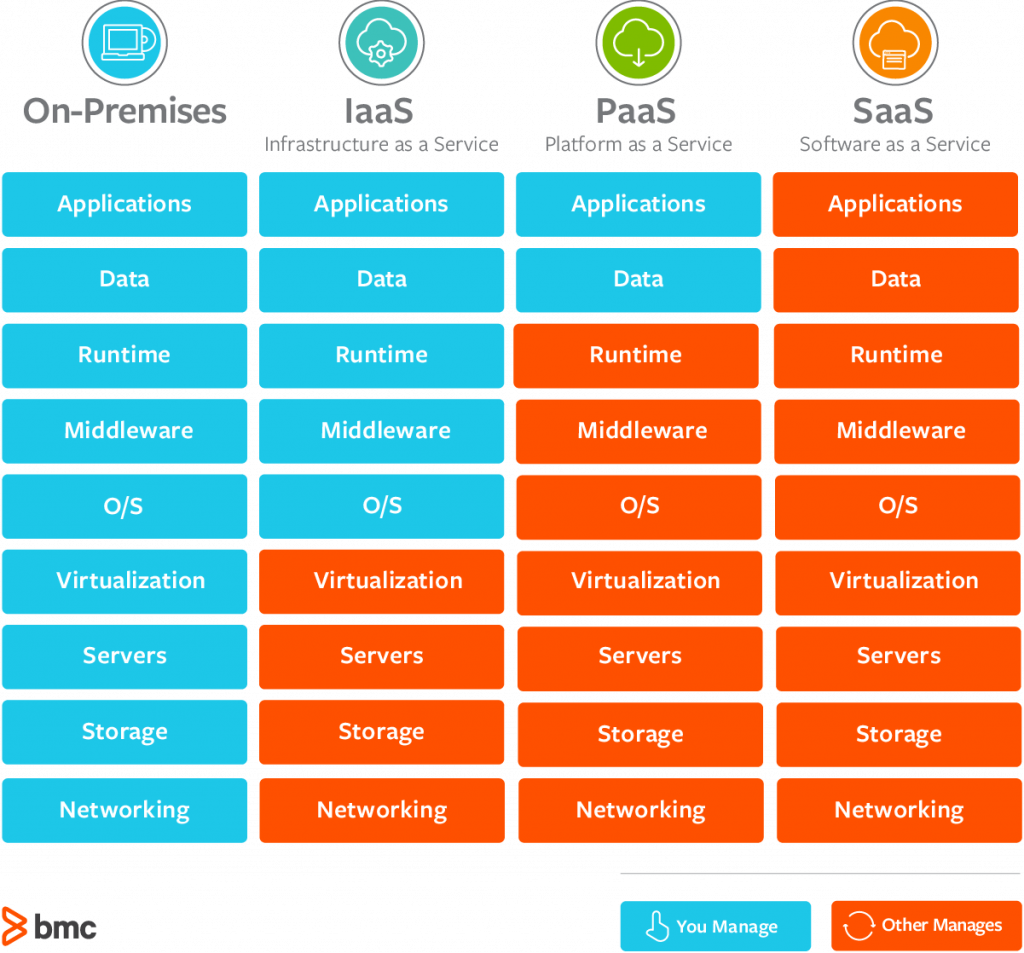
\includegraphics[height=10cm,width=13cm]{presentation/saas-vs-paas-vs-iaas-1024x953}}
    \end{center}

    \caption{ Différents architecture entre SaaS ,PaaS et IaaS}
\end{figure}
\subsubsection{\fontfamily{ptm}\selectfont\Large Les modèles de déploiement }

Il existe 3 modèles de déploiement sur le cloud:

\par \noindent \textbf{\Large -Cloud Privé:  } Le cloud privé est un modèle informatique qui offre un environnement propriétaire dédié à une seule entité commerciale. Comme les autres types d'environnements du cloud computing, le cloud privé fournit des ressources informatiques étendues et virtualisées via des composants physiques stockés sur place ou dans le centre de données d'un fournisseur\cite{6}.\\[0.1cm]

\noindent \textbf{\Large -Cloud Public: } Le cloud public est un type de calcul dans lequel les ressources sont proposées par un fournisseur tiers via Internet, et sont partagées par les organisations et les individus qui souhaitent les utiliser ou les acheter \cite{7}.\\[0.1cm]

\noindent \textbf{\Large -Cloud Hybride :  } Un cloud hybride est un environnement informatique mixte dans lequel des applications s'exécutent à l'aide d'une combinaison de ressources de calcul, de stockage et de services dans différents environnements (clouds publics et clouds privés, y compris des centres de données sur site ou en périphérie)\cite{8}(voir figure 1.5).\\[0.1cm]

\begin{figure}[H]
    \begin{center}
    \fbox{
\includegraphics[height=7cm]{presentation/cloud.png}}
    \end{center}

    \caption{ Différents type du cloud}
\end{figure}

\section{\fontfamily{ptm}\selectfont\Large Méthodologie de développement adoptée}

 Avant de réaliser un projet informatique, il est essentiel de sélectionner une démarche de travail et une procédure de suivi pour obtenir un logiciel stable. Il s'agit d'un cadre permettant de structurer, de planifier et de contrôler le développement d'une application.\\
Pour la réalisation de notre projet nous avons opté pour la méthodologie agile SCRUM car elle
améliorer la flexibilité de projet et réduit le temps de livraison de produits complet au client.En
effet , la plupart des projets réalisés dans l’entreprise appliquent cette méthodologie.
 \\[0.2cm]


%\begin{figure}[H]
%    \begin{center}
        %taille de l'image en largeur
        %remplacer "width" par "height" pour régler la hauteur
%    \fbox{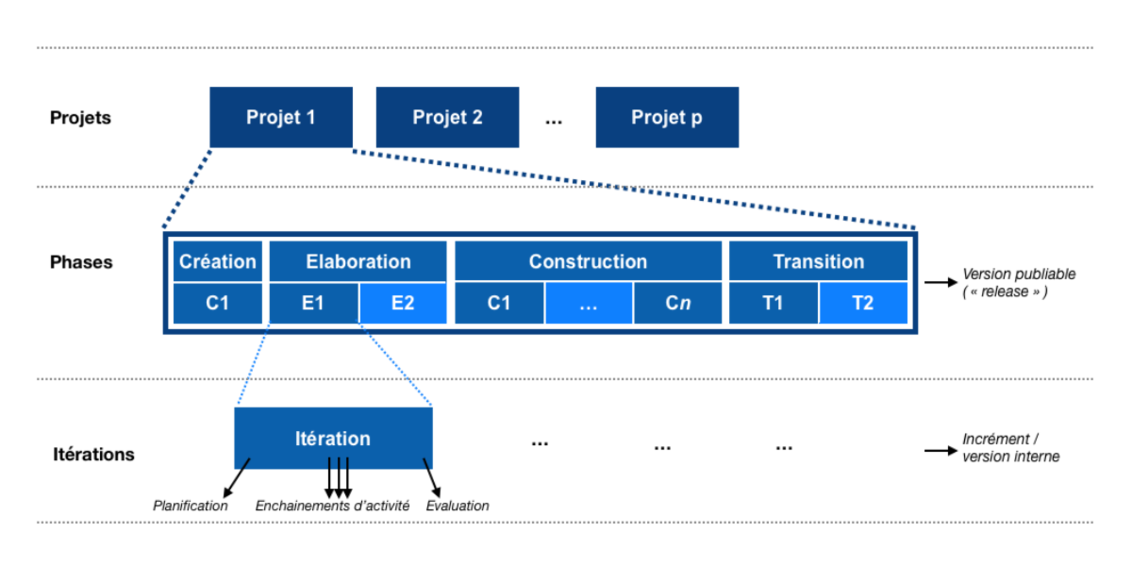
\includegraphics[height=6cm]{2 tracks unified process}}
%    \end{center}
    %légende de l'image
%    \caption{Cycle de vie de projet avec le processus unifié }
%\end{figure}
%\texttt{}\\[0.2cm]
\subsection{\fontfamily{ptm}\selectfont\Large Méthode agile }

Agile est une méthode de gestion de projet conçue pour distribuer en continu les logiciels opérationnels en fonction d'itérations rapides. Il permet aux équipes de développer progressivement un produit de qualité et d'adapter leur processus en fonction des besoins du projet.


\subsection{\fontfamily{ptm}\selectfont\Large  Présentation de la méthodologie Scrum}
\texttt{}\\[0.2cm]

Scrum est une méthodologie agile pour l'élaboration, la réalisation et le soutien de projets complexes. Elle est basée sur la division du produit sur différentes itération sprints.
Scrum est plus utile lorsque les exigenes sont variables et peuvent changer beaucoup de fois au cours du cycle de vie, ce qui donne donc la capacité d'avoir un projet flexible capable de traiter les changements fréquents.
\subsection{\fontfamily{ptm}\selectfont\Large    Acteurs de la méthode agile Scrum}
\texttt{}\\[0.2cm]

Méthode agile Scrum se compose par 3  acteurs ce suit:
\par \noindent \textbf{\Large -Scrum Master: } Il s'agit de la personne chargée d'orienter l'équipe de travail vers la bonne voie, d'assurer la bonne pratique des règles de la méthode Scrum et d'organiser son équipe. \\[0.1cm]

\noindent \textbf{\Large -Product Owner: } il représente les clients et assure que leurs besoins et visions soient réalisés dans le projet. Il travaille généralement en collaboration directe avec l’équipe de développement. \\[0.1cm]

\noindent \textbf{\Large -Equipe de développement: }sont les personnes responsables de la transformation des besoins du client. Ces besoins sont définis par le Product Owner à travers des fonctions utilisables. L'équipe est composée d'au moins 3 personnes jouant les rôles de développeur ou de concepteur.\\[0.1cm]
\subsection{\fontfamily{ptm}\selectfont\Large Évènements de la méthode agile Scrum }

 Scrum définit cinq types d'évènements :\\[0.1cm]%????????????????
\par \noindent \textbf{\Large -Le sprint: }Chaque sprint est de durée maximale de 4 semaines pendant laquelle une version de produit est réalisée. Une fois un sprint terminé un nouveau a déjà commencé avec une liste de fonctionnalités et un objéctif à réaliser. \\[0.1cm]

\noindent \textbf{\Large -Planification d’un sprint: }À chaque début de sprint, cette réunion est conçue pour déterminer les tâches à réaliser pendant le sprint. L’organisation de ces tâches est effectuée par l’équipe de développement et le Product Owner. \\[0.1cm]

\noindent \textbf{\Large -Mêlée quotidienne: } C'est une réunion d'une durée de 15 minutes faite par l’équipe chaque jour pour définir l’objectif de la journée et identifier les obstacles s’il y en a quelques-uns.\\[0.1cm]

\noindent \textbf{\Large -Revue de sprint: }  Représente le travail réalisé par l’équipe au cours du sprint et le comparer avec le produit attendu.\\[0.1cm]

\noindent \textbf{\Large -Rétrospective de sprint: } Le but de cet événement est de déterminer les problèmes intervenus dans la période du sprint, l’efficacité des outils et déterminer ce qui peut être amélioré.

\subsection{ \fontfamily{ptm}\selectfont\Large Les artefacts}

\noindent \textbf{\Large -Product Backlog: }
  Il s’agit d’une liste des besoins et exigences à recueillir pour créer le produit désiré, ce document est la responsabilité de Product Owner(voir figure 1.6).\\[0.1cm]

\noindent \textbf{\Large -Sprint Backlog: } C’est l’ensemble des données permettant la réalisation des objectifs du sprint. Ce document est mis à jour par l’équipe de développement régulièrement.

\begin{figure}[H]
    \begin{center}
        %taille de l'image en largeur
        %remplacer "width" par "height" pour régler la hauteur
    \fbox{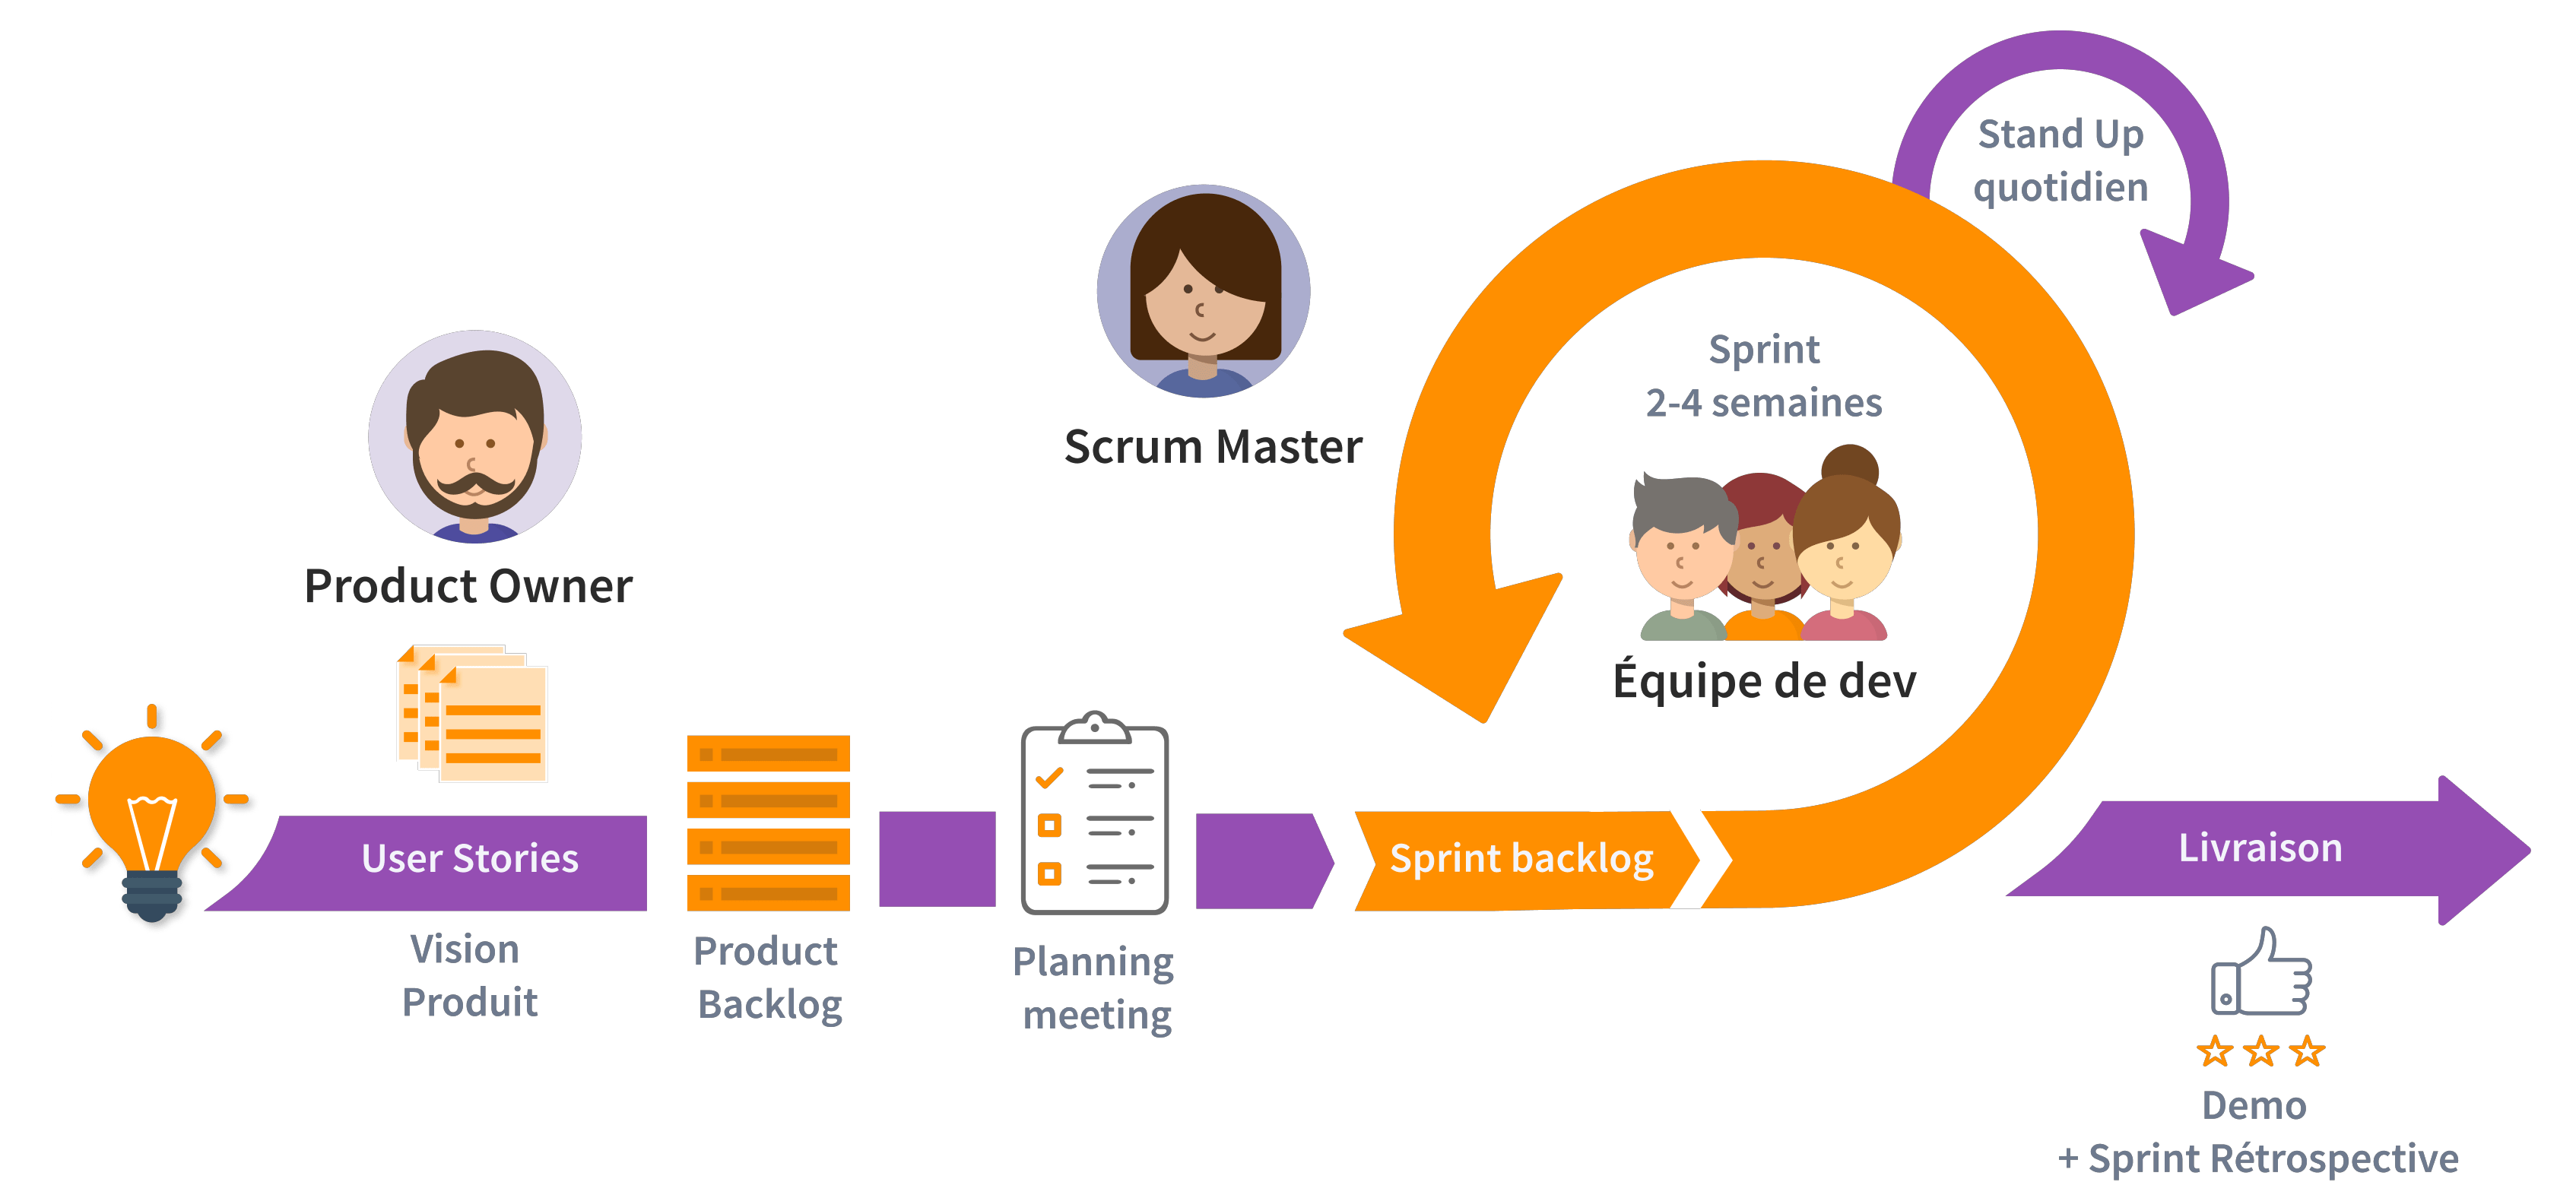
\includegraphics[height=7cm]{agile-Scrum-sprint-workflow-schema-FR.png}}
    \end{center}
    %légende de l'image
    \caption{Processus de méthode Scrum}
\end{figure}


\section{\fontfamily{ptm}\selectfont\Large Planification des sprints}
 
Pour une meilleure optimisation  du développement du projet nous avons divisé le travail en des Sprints présentés dans un diagramme de Gantt qui décrit l’état d’avancement dans le temps des différentes activités (voir figure 1.7):

\begin{figure}[H]
    \begin{center}
        %taille de l'image en largeur
        %remplacer "width" par "height" pour régler la hauteur
    \fbox{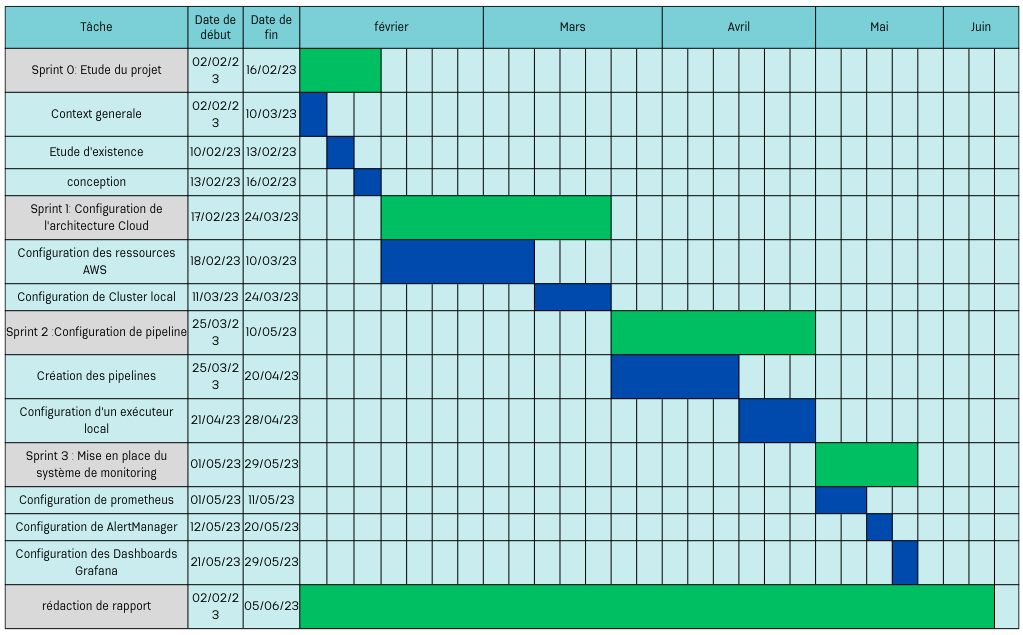
\includegraphics[height=11cm]{presentation/Gantt.png}}
    \end{center}
    %légende de l'image
    \caption{Diagramme de Gantt}
\end{figure}
\section{\fontfamily{ptm}\selectfont\Large Les solutions existantes}

 On va passer  en revue les solutions similaires à notre solution. Nous allons étudier les points forts ainsi que les points faibles de ces solutions afin de montrer pourquoi nous devrions developper notre propre solution. Voici une présentation de certaines solutions existantes :
\subsection{\fontfamily{ptm}\selectfont\Large Azure Devops}
Azure DevOps prend en charge une culture collaborative et un ensemble de processus qui rassemblent les développeurs, les responsables de projets et les contributeurs pour développer des logiciels. Elle permet aux organisations de créer et d’améliorer les produits à un rythme plus rapide que possible avec les approches traditionnelles de développement de logiciels.Azure DevOps Services vous donne également accès aux serveurs de génération et de déploiement cloud et aux insights sur les applications. Démarrez gratuitement et créez une organisation. Ensuite, chargez votre code pour partager ou contrôler le code source. Commencez à suivre votre travail à l’aide de Scrum, Kanban ou d’une combinaison de méthodes \cite{9} (voir figure 1.8).
Elle a des points forts mais aussi des points faibles:\\[0.2cm]
\textbf{\Large\indent

\begin{tikzpicture}
   \draw[fill=black] (2,2) circle (2pt);
 \end{tikzpicture} Points forts:}
\par \indent 
-- Azure DevOps offre une haute disponibilité,sécurité solide et offre de bonnes options d’évolutivité.\\[0.02cm]
\indent-- Azure DevOps est un outil informatique qui adapter en fonction des exigences du projet sans problème,offre a l'utilisateur une flexibilité en matière de gestion de l’infrastructure.\\[0.2cm]
\textbf{\Large\indent

\begin{tikzpicture}
   \draw[fill=black] (2,2) circle (2pt);
 \end{tikzpicture}  Points faibles:}
\par \indent 
-- Azure DevOps propose de nombreuses fonctions prêtes à l'emploi, mais la personnalisation peut être limitée. Les organismes ayant des besoins spéciaux peuvent avoir de la difficulté à adapter l'outil à leurs besoins précis.\\[0.02cm]
\indent-- Azure DevOps fonctionné particulièrement sur cloud qui nécessite une connexion internet pour fonctionner, l'absence d'accès hors ligne peut constituer un inconvénient dans les situations où les personnes doivent travailler à distance avec une connectivité Internet limitée. 
\begin{figure}[H]
    \begin{center}
    
        \fbox{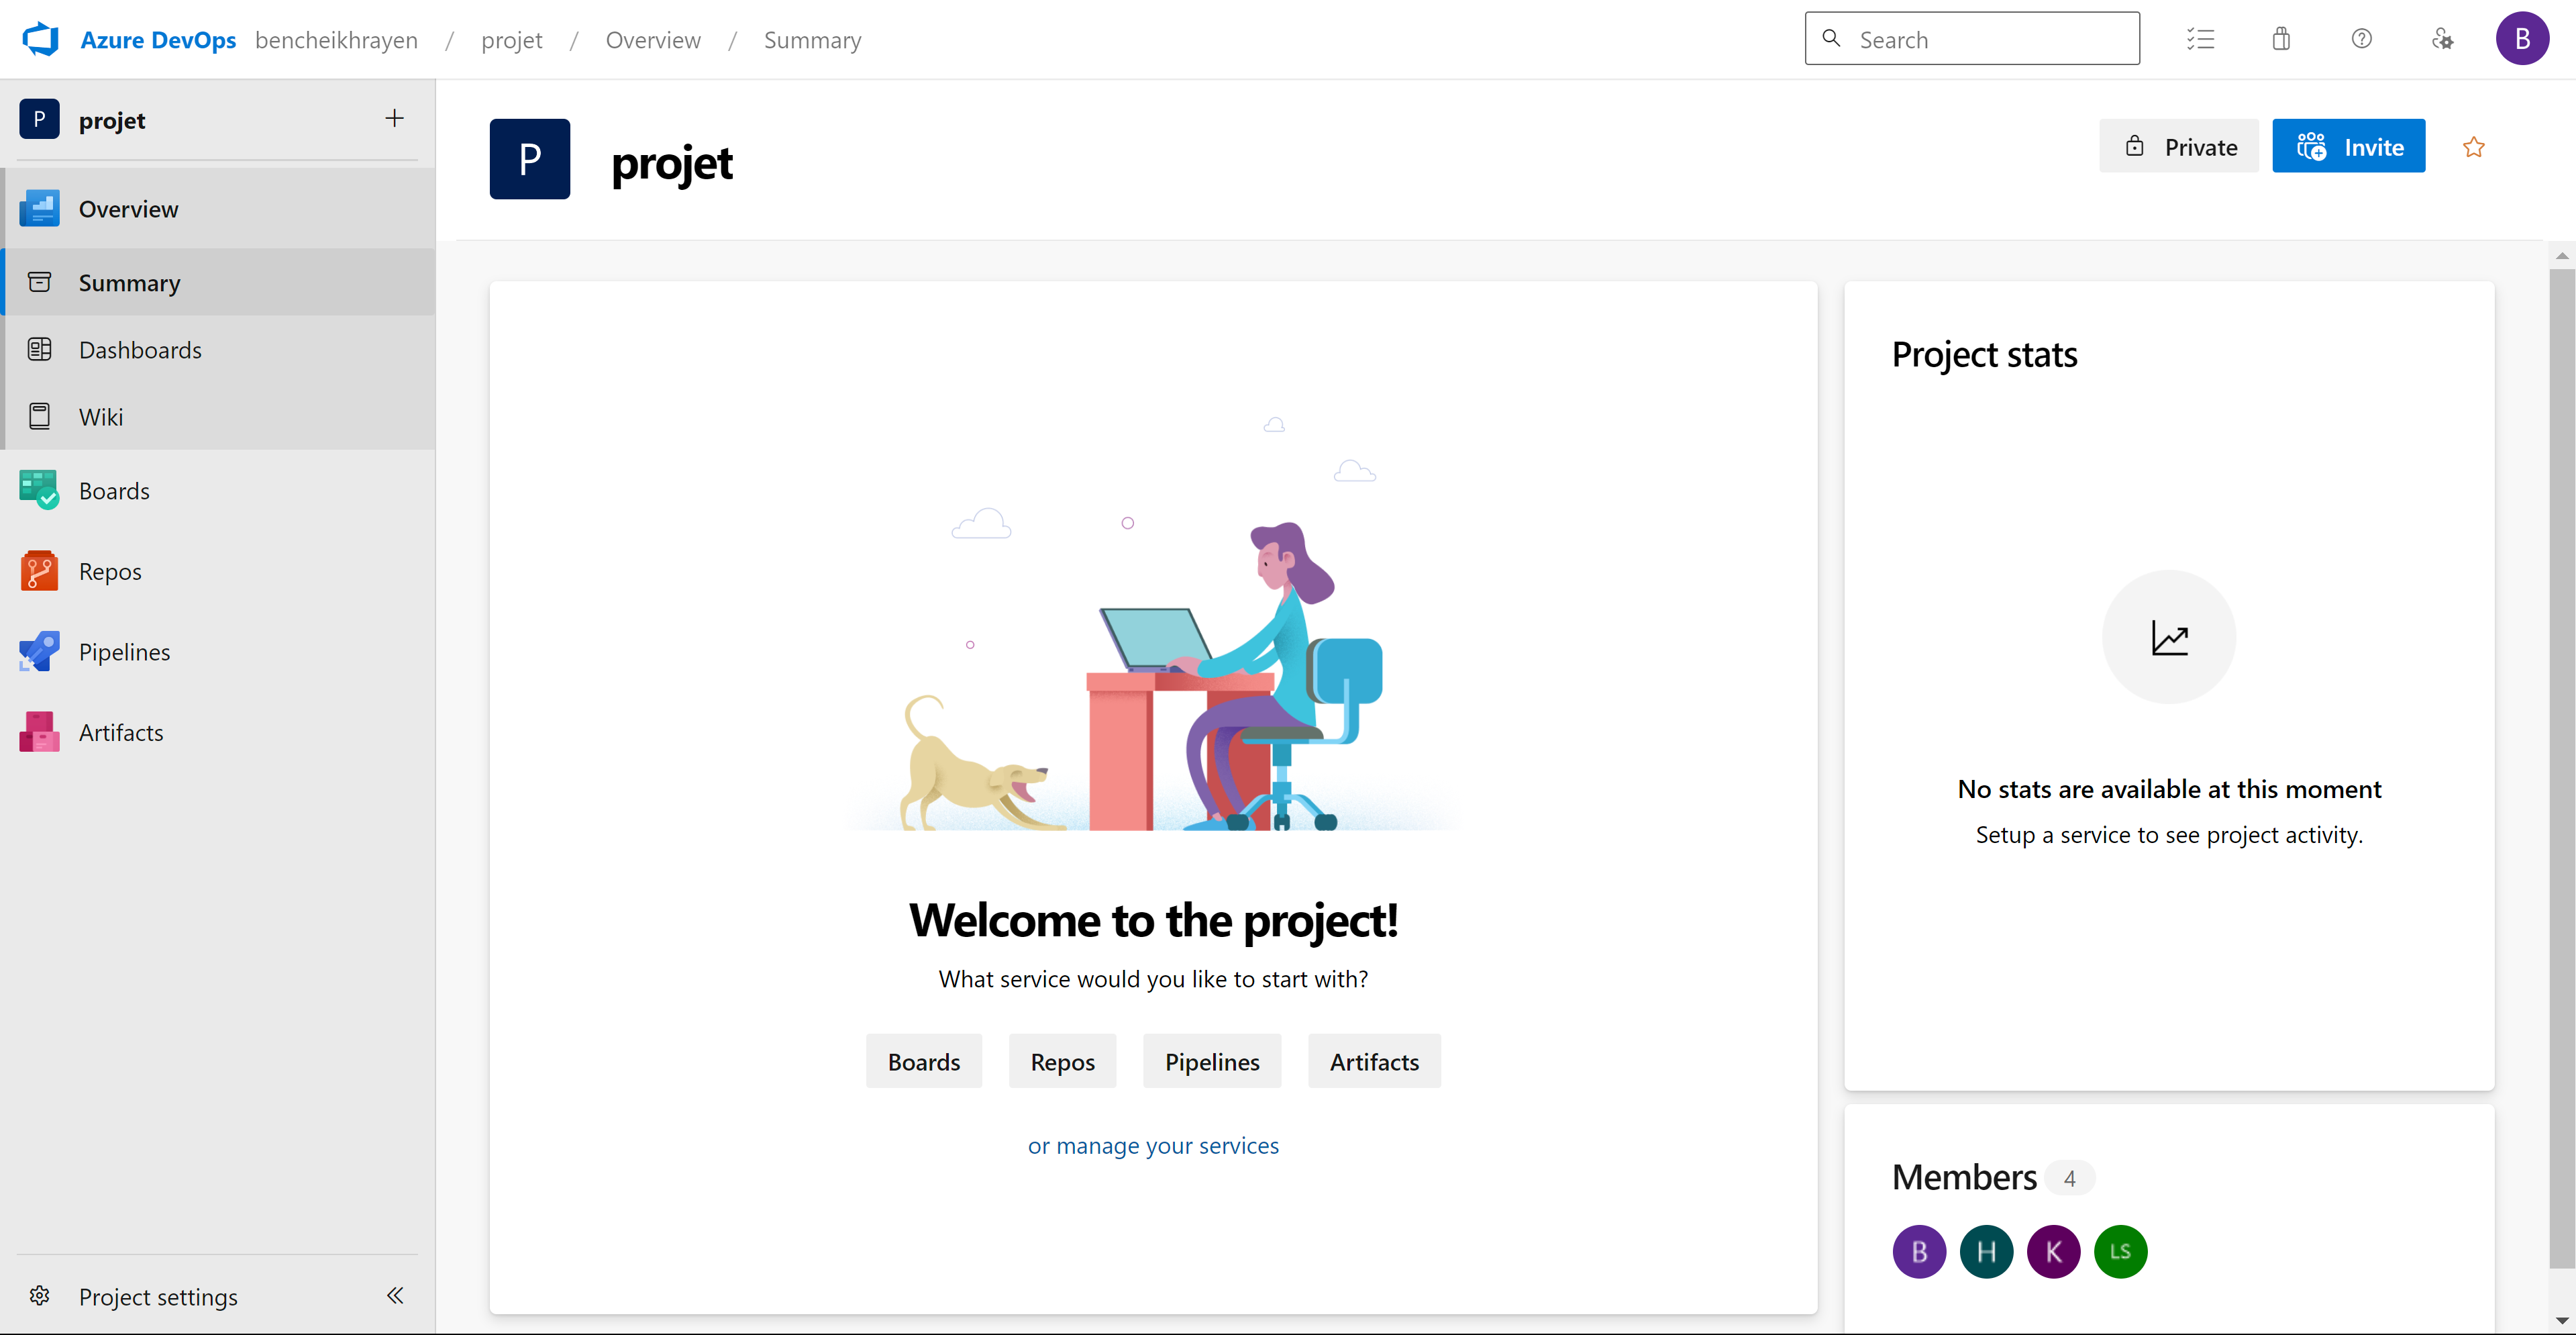
\includegraphics[height=9cm]{azure.png}}

    \end{center}
    
    \caption{Azure DevOps}
\end{figure}

\subsection{\fontfamily{ptm}\selectfont\Large Amazon Web Service DevOps}

 AWS fournit un ensemble de services flexibles, conçus pour permettre aux entreprises de créer et livrer des produits avec plus de rapidité et de fiabilité à l'aide d'AWS et des pratiques de DevOps. Ces services simplifient la mise en service et la gestion de l'infrastructure, le déploiement de code d'application, l'automatisation des processus de publication de logiciel et le suivi des performances de l'application et de l'infrastructure \cite{10}(voir figure 1.9).\\Cependant, comme toute autre technologie, AWS présente sur des points forts et des points faibles:\\[0.1cm]
 \textbf{\Large\indent
 
\begin{tikzpicture}
    \draw[fill=black] (2,2) circle (2pt);
  \end{tikzpicture} Points forts:}
 \par \indent {-- Aws offre une grande évolutivité pour les entreprises peuvent facilement augmenter ou réduire leurs ressources en fonction de leurs besoins .Aussi il présente un niveau de fiabilité élevé et il fournit aux entreprises une gamme de services, notamment le stockage, la gestion de bases de données, la puissance de calcul et l’analyse\\[0.02cm]
 \indent-- AWS fournit des outils de redondance et de tolérance aux défaillances, tels que l'auto-scaling et la disponibilité de plusieurs zones. Ces caractéristiques renforcent la disponibilité des applications et assurent des performances fiables. }\\[0.01cm]
\textbf{\Large\indent

\begin{tikzpicture}
   \draw[fill=black] (2,2) circle (2pt);
 \end{tikzpicture} Points faibles:}
\par \indent{-- AWS est complexe à mettre en place et à gérer ses ressources. Aussi, les entreprises doivent prendre des mesures pour garantir la protection de leurs données.\\[0.02cm]
\indent-- L'adoption d'AWS DevOps peut créer une dépendance envers les differents services, ce qui peut mener à un verrouillage des fournisseur. }
\begin{figure}[H]
  \begin{center}
  
      \fbox{\includegraphics[width=15cm]{AWS.png}}

  \end{center}
  
  \caption{Les Services AWS utilisé pour DevOps. }
\end{figure}
\subsection{\fontfamily{ptm}\selectfont\Large Google Cloud Platform DevOps }
Google propose de nombreux services et fonctionnalités visant à aider les ingénieurs DevOps à disposer de tout ce dont ils ont besoin pour respecter les normes de qualité et de sécurité les plus élevées tout en automatisant la majorité du processus.De plus, vous travaillez avec des outils GCP DevOps efficaces qui non seulement augmentent la qualité des applications, mais améliorent également la vitesse du cycle de développement. Ces outils DevOps s’adressent directement aux ingénieurs logiciels car ils permettent une configuration rapide et simple, avec une interface intuitive qui facilite l’utilisation efficace des outils et méthodologies de livraison continue et de déploiement continu (intégration continue/ déploiement continu(CI/CD))\cite{11}(Voir figure 1.10).\\Ainsi GCP a des points forts et des points faibes:\\[0.2cm]
 \textbf{\Large\indent
 
\begin{tikzpicture}
    \draw[fill=black] (2,2) circle (2pt);
  \end{tikzpicture} Points forts:}
 \par\indent
  -- GCP fournit des services d'intégration et de développement d'applications et assure une bonne sécurité.\\[0.02cm]
 \indent-- GCP DevOps rendre facile la collaboration entre les équipes de développement et les équipes opérationnelles grâce à des services partagés.
 \\[0.2cm]
\textbf{\Large\indent

\begin{tikzpicture}
   \draw[fill=black] (2,2) circle (2pt);
 \end{tikzpicture} Points faibles:}
\par\indent
-- Quelque intégration peut être plus limitées avec les services et les outils de Google par rapport à des solutions locales. De plus, la configuration initiale du GCP est complexe en raison de la grande diversité de services et d'options disponibles.\\[0.02cm]
\indent-- L'utilisation efficace de GCP DevOps exige un personne qualifié spécialisé dans les technologies cloud, l'automatisation et la gestion de l'infrastructure.
\\[0.1cm]
\begin{figure}[H]
  \begin{center}
  
      \fbox{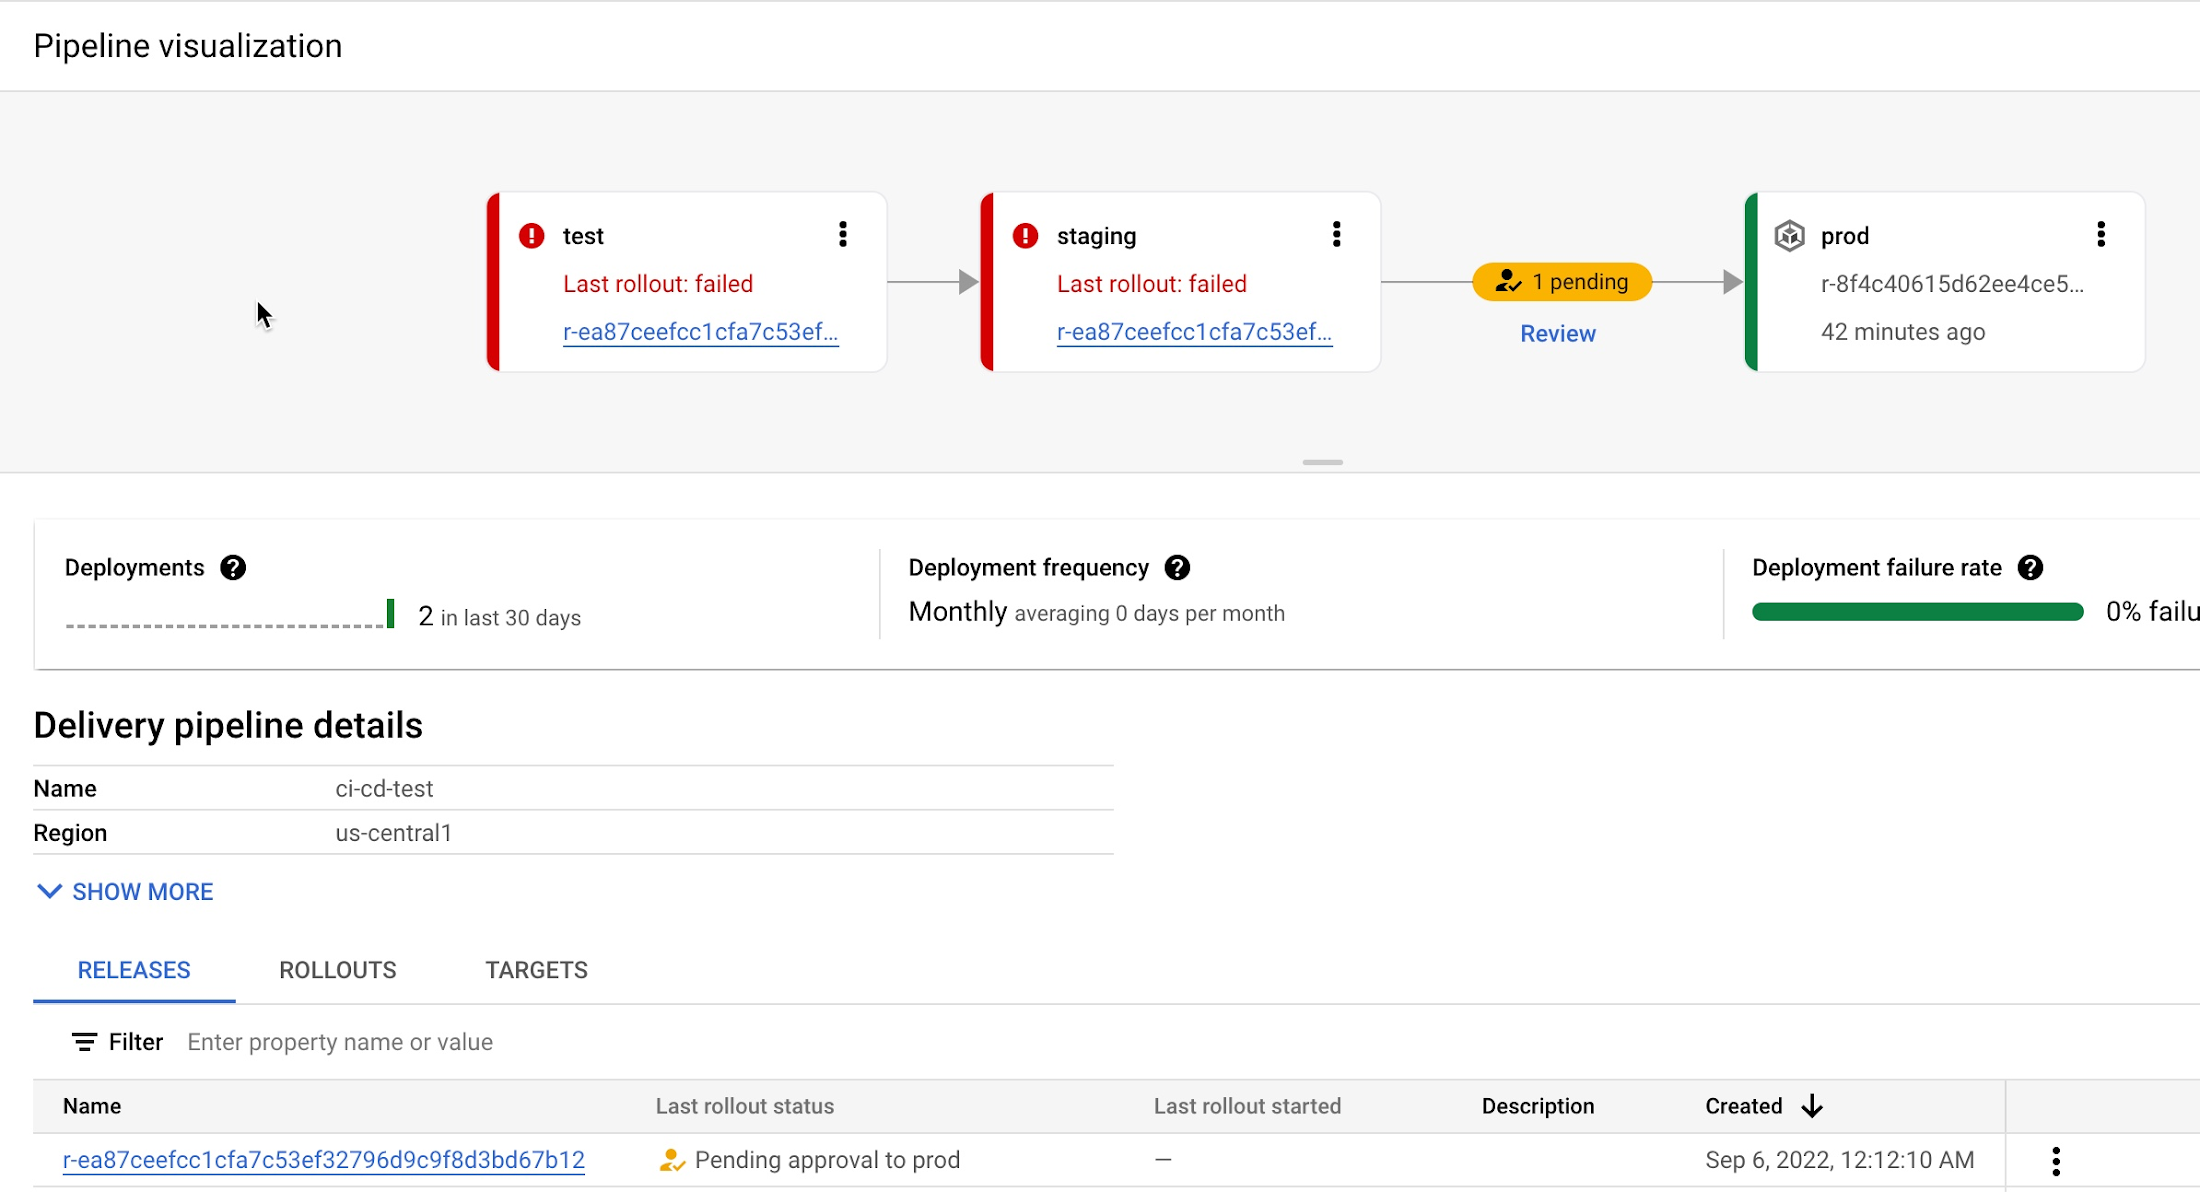
\includegraphics[width=15cm]{presentation/GPC.png}}

  \end{center}
  
  \caption{Interface de GCP Pipeline.}
\end{figure}
\section{\fontfamily{ptm}\selectfont\Large Critique des solutions existantes}

Nous allons comparer les solutions présentées ci-dessus selon plusieur critères qu'on va définir par rapport aux besoins de l'entreprise(voir tableau 1.1).\\
\par \noindent \textsf{\fontfamily{ptm}\selectfont\scalefont{1.3} C1 -La confidentialité des données d'application : } La solution doit privilégier la confidentialité des données puisque certains clients préfèrent leur application exécutée sur le serveur local de la société. \\[0.1cm]
\noindent \textsf{\fontfamily{ptm}\selectfont\scalefont{1.3} C2 -Intégration de solutions source libre: } Amazon cloud, azure cloud ou toute autre solution cloud doit intégrer certaines software open source comme services à utiliser dans votre architecture cloud.Bien que les logiciels libres puissent être hautement personnalisables, le niveau de personnalisation fourni par un fournisseur de services peut être restreint. \\[0.1cm]
\noindent \textsf{\fontfamily{ptm}\selectfont\scalefont{1.3} C3 -Coût de projet : } L'utilisation d'Amazon Cloud ainsi tout autre fournisseur pour  déployer une application dans le Cloud semble peu coûteux au début, mais après que la charge de travail augmente, les coûts aussi augmentent. Il s'agit de trouver une solution qui profite du cloud et des avantages du logiciel libre.\\[0.1cm]
\noindent \textsf{\fontfamily{ptm}\selectfont\scalefont{1.3} C4 -Problèmes de compatibilité: } La personnalisation peut présenter des problèmes de compatibilité, surtout si la personnalisation interagit avec d'autres services ou composants au cours du déploiement. Cela peut entraîner des temps d’arrêt ou d’autres problèmes de performance.\\[0.5cm]
\begin{center}
  \begin{table}
\centering
\begin{tabular}{|c|c|c|c|}
\hline
 & Azure DevOps & Amazon Web Service DevOps & Google Cloud Platform DevOps \\
\hline
C1 & \textbf{X} & \textbf{X} & \textbf{X} \\
\hline
C2 & \checkmark & \checkmark & \checkmark \\
\hline
C3 & \checkmark & \checkmark & \textbf{X} \\
\hline
C4 & \textbf{X} & \textbf{X} & \textbf{X} \\
\hline
\end{tabular}

\medskip

\begin{flushright}
\fbox{\parbox{0.5\linewidth}{%
\textsf{\fontfamily{ptm}\selectfont\scalefont{1.3} Légende: \\
X: La solution ne conforme pas à la critère. \\
\checkmark: La solution conforme à la critère.}}}
\end{flushright}

\caption{Tableau comparatif}
\end{table}
\end{center}
 En se basant sur le tableau comparatif ci-dessus, on constate que les solutions basées uniquement sur le cloud ne sont pas utiles, et qu'une combinaison de ressources cloud et locales est conforme à notre projet.\\[0.1cm]
Notons que cette évaluation ne concerne que notre situation, dans d'autres cas les solutions existantes peuvent être utile.  

%tableau centré à taille variable qui s'ajuste automatiquement suivant la longueur du contenu
\section{\fontfamily{ptm}\selectfont\Large Solution proposée}%???????????
 Pour rectifier les problèmes auxquels l’équipe DevOps fait face chaque jour et afin de  préparer un environnement de développement flexible, Mobelite nous a proposé de mettre en place une solution Hybride cloud qui bénéficie à la fois  de certain services de cloud avec un accès privé aux données. En effet, le projet consiste à implémenter la conteneurisation qui nous offrira une virtualisation des ressources de manière légère, flexible et puissante. Le déploiement d’un kubernetes cluster qui est un système de gestion de conteneurs qu'on va utiliser pour optimiser le déploiement des applications avec l’utilisation d’autres produits comme Ansible pour l’optimisation de cette infrastructure. La solution a des objectifs importants pour l’entreprise comme la réduction des coûts de développement et d'exploitation. Le Cycle de développement sera plus court grâce à l'automatisation et le déploiement rapide des nouveaux environnements.Aussi, la solution garantira la supervision totale et continue de la plateforme, et la haute disponibilité du système.\\[0.1cm]


\textbf{\huge Conclusion} \\[0.3cm]  

 Dans ce chapitre nous avons présenté la société d’accueil, la problématique et la méthodologie de développement.
    Aussi, nous avons réalisé une étude de quelques solutions existantes,
puis nous avons réalisé une comparaison de l'existant pour connaître les solutions
compatibles avec notre sujet. Après cela, nous avons présenté la solution proposée
par mobelite.